\documentclass[11pt,a4paper]{article}
\usepackage[T1]{fontenc}
\usepackage[utf8]{inputenc}
\usepackage{lmodern}
\usepackage[margin=2cm,top=1.8cm,bottom=2cm]{geometry}
\usepackage{graphicx}
\usepackage{booktabs,tabularx,longtable,array}
\usepackage{amsmath}
\usepackage[table]{xcolor}
\usepackage{listings}
\usepackage{tikz}
\usetikzlibrary{shapes.geometric,arrows.meta,positioning,calc,shapes.misc}
\usepackage{enumitem}
\usepackage{caption}
\usepackage{float}
\usepackage{needspace}
\usepackage[hidelinks]{hyperref}

\setlist{itemsep=1pt,topsep=3pt}
\setlength{\parskip}{3pt}
\newcommand{\code}[1]{\texttt{#1}}
\definecolor{codebg}{gray}{0.96}
\lstset{language=Python,basicstyle=\ttfamily\small,frame=single,backgroundcolor=\color{codebg},
  keywordstyle=\color{blue!60!black}\bfseries,commentstyle=\color{gray}\itshape,
  stringstyle=\color{green!40!black},showstringspaces=false,columns=fullflexible}

% Photo: shows the picture if the file exists, otherwise an empty frame
\newcommand{\photo}[2]{%
  \IfFileExists{#1}{\includegraphics[width=\linewidth,height=4.2cm,keepaspectratio]{#1}}%
  {\fbox{\parbox[c][3.8cm][c]{0.92\linewidth}{\centering\small\color{gray}
   Photo: upload \texttt{#1} to Overleaf\\[2pt]#2}}}}

\tikzset{
  >={Stealth[length=2.2mm]},
  box/.style={draw,rectangle,rounded corners=2pt,align=center,minimum height=7mm,
              minimum width=30mm,font=\small,fill=blue!5},
  term/.style={draw,rounded rectangle,align=center,minimum height=7mm,minimum width=24mm,
               font=\small\bfseries,fill=gray!15},
  dec/.style={draw,diamond,aspect=2.4,align=center,inner sep=1pt,font=\small,fill=orange!10},
  io/.style={draw,trapezium,trapezium left angle=72,trapezium right angle=108,align=center,
             minimum height=7mm,font=\small,fill=green!6},
  lab/.style={font=\scriptsize,midway},
}

\begin{document}

% ------------------------------------------------------------------ title
\begin{titlepage}
\centering
\vspace*{1.5cm}
{\large UFAZ\\[2pt] Algorithms and Programming 1\par}
\vspace{2.2cm}
{\Huge\bfseries Minesweeper in Python\par}
\vspace{0.4cm}
{\large Final project report\par}
\vspace{2.2cm}
{\large
Zeynalzada Ayxan\\[2pt]
Maharramli Anvar\\[2pt]
Qurbanli Elton\\[2pt]
Nuruzada Nihat\\[2pt]
Hamzayev Altair\par}
\vfill
{\large November 2026\par}
\end{titlepage}

\tableofcontents
\vspace{6mm}
\noindent\textbf{How to run.} Python 3.7 or later, nothing to install. Keep all \code{.py} files in one
folder and type \code{python main.py}. For the demonstration: level 1, seed 7, first move \code{R E5}
gives exactly the example screen of the assignment.
\vspace{4mm}

% ------------------------------------------------------------------ 1
\section{Overview}

We wrote a text version of Minesweeper in Python. The player sees a hidden grid, reveals cells with
commands such as \code{R E5}, and must open every cell without a mine. The program uses only what was
seen in the course: variables, conditions, loops, functions, strings, lists (and lists of lists),
tuples, sets and dictionaries. There is no object-oriented programming and the only modules imported
are \code{random} and \code{time}.

\subsection{Rules as we implemented them}
\begin{itemize}
\item \textbf{Board.} Columns are letters (A, B, C, \dots), rows are numbers starting at 1; a cell is
  written \code{C4}. Inside the program a cell is the tuple \code{(row, col)} starting at 0, so
  \code{C4} is \code{(3, 2)}.
\item \textbf{Levels.} Easy $9\times9$ with 10 mines, Medium $12\times12$ with 25, Hard $16\times16$ with 40.
\item \textbf{States.} Each cell is hidden (\code{\#}), revealed (\code{.} or \code{1}--\code{8}) or flagged (\code{F}).
\item \textbf{Reveal.} A mine loses the game. Otherwise the cell shows how many of its 8 neighbours
  are mines. A \code{0} opens its neighbours automatically, and so on (flood fill).
\item \textbf{First move.} Mines are placed only after the first reveal and never on that cell.
\item \textbf{Flags.} \code{F C3} puts or removes a flag. A flagged cell cannot be revealed and is
  never opened by the flood fill. The screen shows \emph{Mines left = mines $-$ flags}.
\item \textbf{End.} The game is won when every safe cell is revealed (flags are not needed). At the
  end the full board is shown: \code{*} for mines, \code{X} for the mine that was hit and \code{!} for
  a flag on a cell without a mine (the assignment does not fix this symbol, so we chose \code{!}).
\item \textbf{Commands.} \code{R}, \code{F}, \code{D} (debug: shows the mines, the game goes on),
  \code{H} (help), \code{Q} (stops the current game and returns to the menu). Upper or lower case.
\item \textbf{Seed.} The player may type a seed. If he presses Enter, the program chooses a random
  seed and \emph{shows it}, so every game can be replayed. The same seed and the same first move
  always give the same board.
\item \textbf{Menu.} After a game: new game, replay the last game (same level and seed), or quit.
\item \textbf{Input.} Any wrong input (unknown command, \code{Z99}, \code{E}, \code{5E}, \code{E-5},
  a revealed or flagged cell, \dots) prints a clear message and asks again; the turn is not lost.
\end{itemize}

\subsection{How we worked}
We followed a plan of 18 phases. First we \textbf{played the game} on all levels and noted its
mechanics and tricks (a \code{1} touching only one hidden cell means that cell is a mine; corners have
3 neighbours, edges 5). We also found variants we did \emph{not} implement, such as infinite
Minesweeper (Figure~\ref{fig:infinite}). Then we turned the assignment into a numbered \textbf{checklist of requirements}, did
\textbf{research} on each mechanic (grid in a list of lists, neighbour offsets, mine placement with a
seed, stack versus recursion), agreed on a \textbf{design} (four files, one state dictionary, the
function table of Section~\ref{sec:design}), wrote the code, \textbf{tested} it, reviewed each other's
files and finally added optional extras.

\begin{figure}[H]
\centering
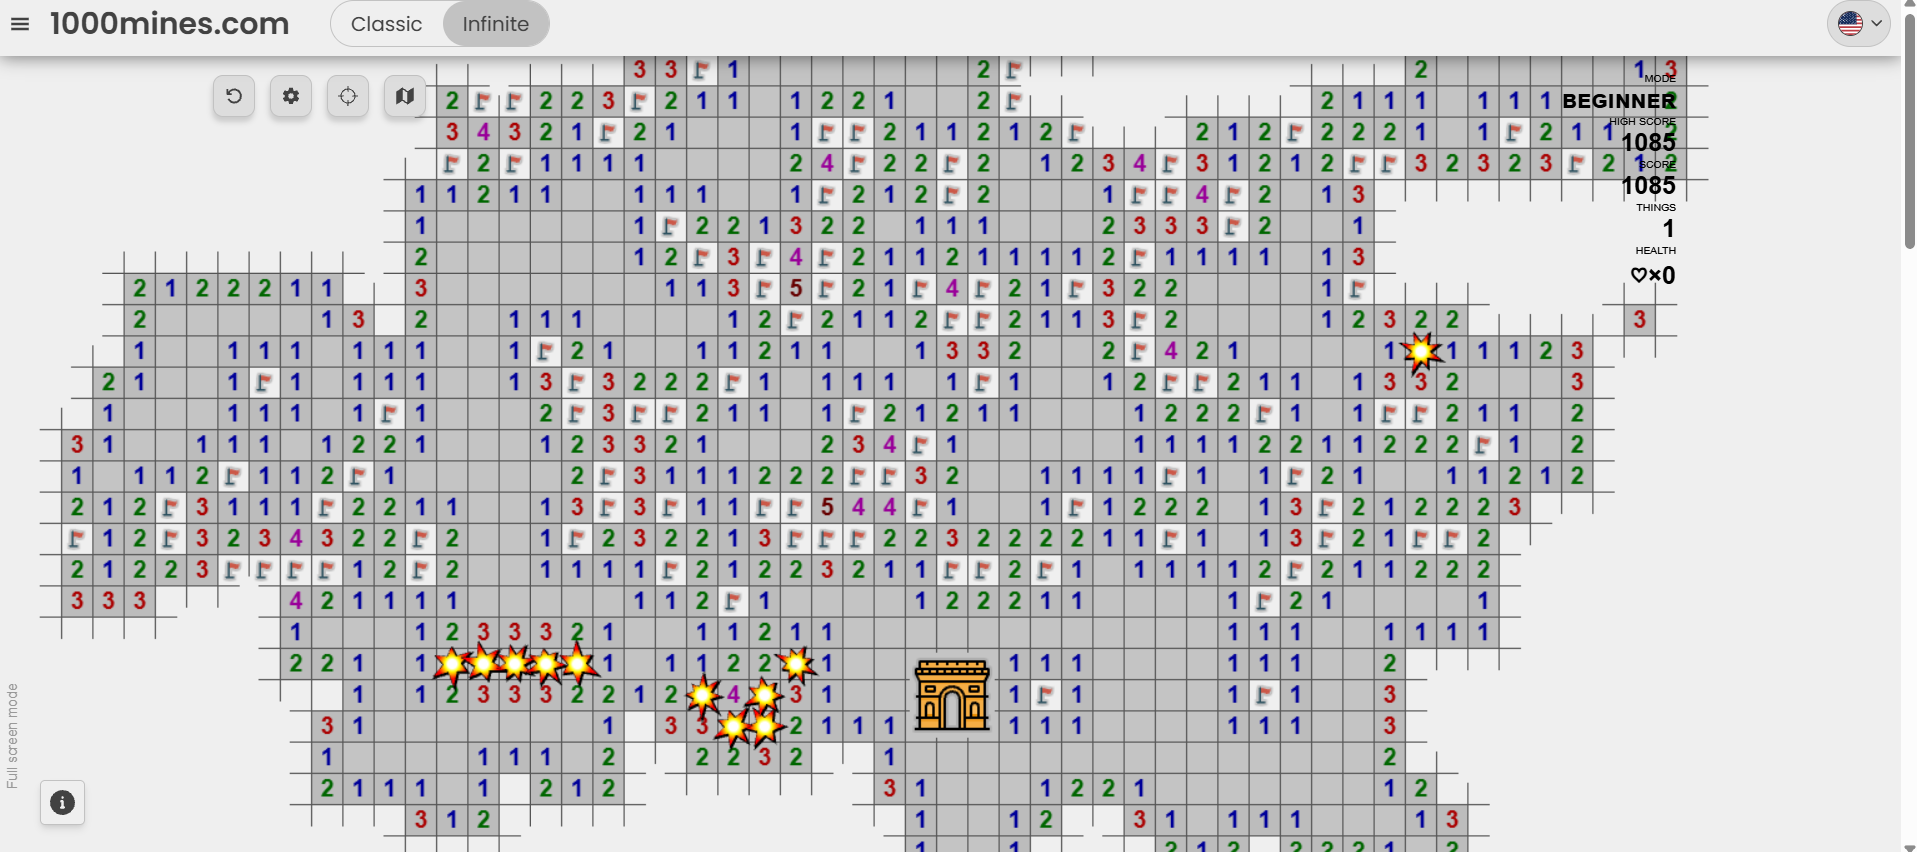
\includegraphics[width=0.8\linewidth]{photos/infinite_minesweeper.png}
\caption{A variant found while studying the game: infinite Minesweeper on 1000mines.com. It was not implemented.}
\label{fig:infinite}
\end{figure}

\begin{figure}[H]
\centering
\begin{minipage}{0.48\linewidth}\centering
\photo{photos/photo1.jpg}{Studying the game together}
\captionof{figure}{Studying the game together.}
\end{minipage}\hfill
\begin{minipage}{0.48\linewidth}\centering
\photo{photos/photo2.jpg}{Team working session}
\captionof{figure}{Team working session.}
\end{minipage}
\end{figure}

% ------------------------------------------------------------------ 2
\section{Design}\label{sec:design}

\subsection{Files}
The code is split into five files. Imports go in one direction only:
\code{main} $\rightarrow$ \code{game\_logic} $\rightarrow$ \code{interface} $\rightarrow$ \code{board}
(\code{scores} is an optional extra used by \code{main}).

\begin{center}
\begin{tabularx}{\linewidth}{l X}
\toprule
\textbf{File} & \textbf{Content} \\
\midrule
\code{board.py} & constants (symbols, levels), board, mines, neighbours, numbers \\
\code{interface.py} & level and seed choice, display, command parsing, help \\
\code{game\_logic.py} & game state, reveal (flood fill), flags, win and loss, one full game \\
\code{main.py} & entry point and menu: new game, replay, quit \\
\code{scores.py} & \emph{extra}: best times in a dictionary, saved in \code{scores.txt} \\
\bottomrule
\end{tabularx}
\end{center}

\subsection{Data structures}
\begin{itemize}
\item \textbf{Board} -- a \emph{list of lists} of one-character strings: \code{board[r][c]} is the
  symbol the player sees (\code{\#}, \code{F}, \code{.}, \code{1}--\code{8}).
\item \textbf{Numbers} -- a list of lists of integers: \code{numbers[r][c]} is the number of
  neighbouring mines, computed once after the first move.
\item \textbf{Mines} -- a \emph{set of tuples} \code{(row, col)}. Testing \code{cell in mines} takes
  constant time on average, which matters because it is done for every neighbour of every cell.
\item \textbf{Revealed cells and flags} -- two more sets of tuples.
\item \textbf{Game state} -- one \emph{dictionary} passed to the functions, so the program has no
  global variable (only constants in capitals):
\end{itemize}
\begin{lstlisting}
state = {"rows": 9, "cols": 9, "nb_mines": 10, "seed": 7,
         "board": [...], "numbers": [...], "mines": {(0, 6), ...},
         "revealed": set(), "flags": set(), "first_move": True,
         "game_over": False, "won": False, "hit_mine": None}
\end{lstlisting}
\begin{itemize}
\item \textbf{Levels} -- the dictionary \code{LEVELS = \{1: (9, 9, 10), 2: (12, 12, 25), 3: (16, 16, 40)\}}.
\item \textbf{Neighbours} -- computed by \emph{one} function, \code{neighbours()}, used by
  \code{count\_adjacent}, \code{reveal} and \code{find\_hint}.
\end{itemize}

\subsection{Function table}
{\footnotesize
\begin{longtable}{>{\ttfamily}p{2.9cm} p{5.6cm} p{4.2cm} p{2.8cm}}
\toprule
\textrm{\textbf{Function}} & \textbf{Role} & \textbf{Parameters} & \textbf{Result} \\
\midrule
\endhead
\multicolumn{4}{l}{\textit{board.py}}\\
create\_board & builds the hidden board & rows, cols & list of lists of \code{\#} \\
neighbours & valid neighbours of a cell (3, 5 or 8) & row, col, rows, cols & list of tuples \\
place\_mines & random mine positions, never on the safe cell & rows, cols, nb\_mines, safe\_cell & set of tuples \\
count\_adjacent & mines around one cell & row, col, mines, rows, cols & int 0--8 \\
compute\_numbers & count\_adjacent for every cell & mines, rows, cols & list of lists of int \\
\midrule
\multicolumn{4}{l}{\textit{interface.py}}\\
is\_number & text made only of digits 0--9 & text & bool \\
choose\_level & asks level and seed, repeats until valid & -- & (rows, cols, nb\_mines, seed) \\
cell\_symbol & symbol of one cell (debug / end shows mines) & cell, state, show\_mines & str \\
display\_board & prints letters, numbers, grid, mines left & state, show\_mines & None \\
parse\_cell & \code{"C4"} $\rightarrow$ \code{(3, 2)} with checks & text, rows, cols & (cell, "") or (None, message) \\
parse\_command & checks one typed line, never crashes & text, rows, cols & (command, cell) or (None, message) \\
show\_help & prints commands and symbols & -- & None \\
\midrule
\multicolumn{4}{l}{\textit{game\_logic.py}}\\
new\_state & creates the state dictionary & rows, cols, nb\_mines, seed & dict \\
start\_mines & seeds \code{random}, places mines, computes numbers at the first reveal & cell, state & None \\
reveal & reveals a cell; flood fill with a while loop and a stack & cell, state & error message or "" \\
toggle\_flag & puts or removes a flag & cell, state & error message or "" \\
check\_win & all safe cells revealed? & state & bool \\
check\_loss & a mine was hit? & state & bool \\
cell\_name & \code{(3, 2)} $\rightarrow$ \code{"C4"} & cell & str \\
play\_game & the game loop of one game & settings & time if won, else None \\
\midrule
\multicolumn{4}{l}{\textit{main.py}}\\
ask\_menu & shows the menu, returns a valid choice & can\_replay & "1", "2", "3" or "4" \\
main & title, then menu until the player quits & -- & None \\
\midrule
\multicolumn{4}{l}{\textit{Optional extras (Section~\ref{sec:extras})}}\\
find\_hint & a safe hidden cell, next to the open area if possible & state & tuple or None \\
ask\_number & asks an integer between two limits & question, low, high & int \\
choose\_custom & size and mines of a custom board & -- & (rows, cols, nb\_mines) \\
record\_time & keeps the time of a won game if it is a record & settings, seconds, scores & None \\
board\_key & scoreboard key, e.g. \code{"9x9, 10 mines"} & rows, cols, nb\_mines & str \\
load\_scores / save\_scores & read / write \code{scores.txt} & (scores,) filename & dict / None \\
update\_scores & stores a time if it is the best & scores, key, seconds & bool \\
show\_scores & prints the best times & scores & None \\
\bottomrule
\end{longtable}}

% ------------------------------------------------------------------ 3
\section{Flowcharts}

Figure~\ref{fig:loop} shows \code{main()} and \code{play\_game()} together. Every wrong input goes back
to ``read a command'' without changing the state, so the player never loses a turn; \code{Q} stops the
game and goes back to the menu. Figure~\ref{fig:reveal} shows \code{reveal()}: the flood fill does not use
recursion, a list is used as a stack. \code{stack.pop()} takes the last cell added, and the neighbours
of a \code{0} are pushed with \code{append}.

\begin{figure}[H]
\centering
\begin{minipage}[t]{0.5\linewidth}\centering
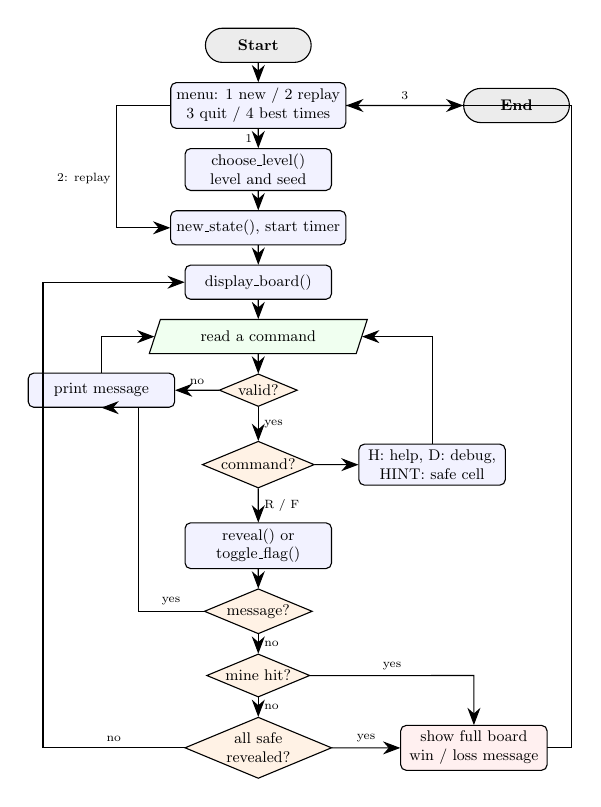
\begin{tikzpicture}[node distance=4mm and 6mm,scale=0.62,transform shape]
\node[term] (start) {Start};
\node[box, below=of start] (menu) {menu: 1 new / 2 replay\\ 3 quit / 4 best times};
\node[box, below=of menu] (level) {choose\_level()\\ level and seed};
\node[box, below=of level] (state) {new\_state(), start timer};
\node[box, below=of state] (show) {display\_board()};
\node[io, below=of show] (read) {read a command};
\node[dec, below=of read] (valid) {valid?};
\node[dec, below=7mm of valid] (cmd) {command?};
\node[box, below=7mm of cmd] (play) {reveal() or\\ toggle\_flag()};
\node[dec, below=of play] (err) {message?};
\node[dec, below=of err] (lost) {mine hit?};
\node[dec, below=of lost] (won) {all safe\\ revealed?};
\node[box, right=14mm of won, fill=red!6] (end) {show full board\\ win / loss message};
\node[box, left=9mm of valid] (msg) {print message};
\node[box, right=9mm of cmd] (info) {H: help, D: debug,\\ HINT: safe cell};
\node[term, right=24mm of menu] (stop) {End};

\draw[->] (start) -- (menu);
\draw[->] (menu) -- node[lab,left]{1} (level);
\draw[->] (level) -- (state);
\draw[->] (state) -- (show);
\draw[->] (show) -- (read);
\draw[->] (read) -- (valid);
\draw[->] (valid) -- node[lab,right]{yes} (cmd);
\draw[->] (valid) -- node[lab,above]{no} (msg);
\draw[->] (msg) |- (read);
\draw[->] (cmd) -- node[lab,right]{R / F} (play);
\draw[->] (cmd) -- (info);
\draw[->] (info) |- ($(read.east)+(0,0)$);
\draw[->] (play) -- (err);
\draw[->] (err.west) -- ++(-1.35,0) node[lab,above]{yes} |- (msg.south);
\draw[->] (err) -- node[lab,right]{no} (lost);
\draw[->] (lost) -- node[lab,above]{yes} (end |- lost) -- (end);
\draw[->] (lost) -- node[lab,right]{no} (won);
\draw[->] (won) -- node[lab,above]{yes} (end);
\draw[->] (won.west) -- ++(-2.9,0) node[lab,above]{no} |- (show.west);
\draw[->] (end.east) -- ++(0.5,0) |- (menu.east);
\draw[->] (menu.east) -- node[lab,above]{3} (stop);
\draw[->] (menu.west) -- ++(-1.1,0) |- node[lab,left,pos=0.3]{2: replay} (state.west);
\end{tikzpicture}
\captionof{figure}{Main game loop.}\label{fig:loop}
\end{minipage}\hfill
\begin{minipage}[t]{0.48\linewidth}\centering
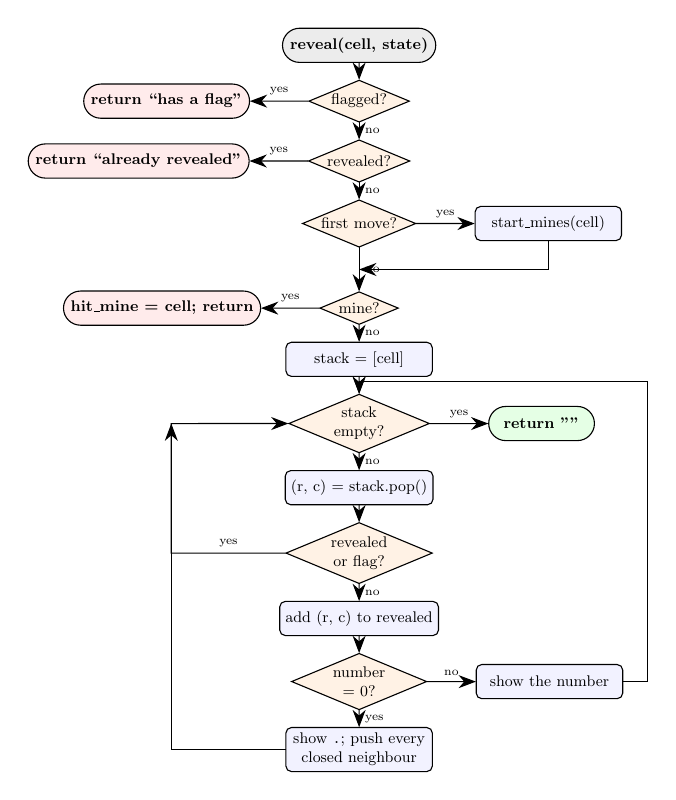
\begin{tikzpicture}[node distance=3.5mm and 6mm,scale=0.62,transform shape]
\node[term] (s) {reveal(cell, state)};
\node[dec, below=of s] (f) {flagged?};
\node[dec, below=of f] (r) {revealed?};
\node[dec, below=of r] (fm) {first move?};
\node[box, right=12mm of fm] (sm) {start\_mines(cell)};
\node[dec, below=9mm of fm] (m) {mine?};
\node[box, below=of m] (st) {stack = [cell]};
\node[dec, below=of st] (e) {stack\\ empty?};
\node[box, below=of e] (p) {(r, c) = stack.pop()};
\node[dec, below=of p] (done) {revealed\\ or flag?};
\node[box, below=of done] (add) {add (r, c) to revealed};
\node[dec, below=of add] (z) {number\\ = 0?};
\node[box, right=10mm of z] (num) {show the number};
\node[box, below=of z] (push) {show \code{.}; push every\\ closed neighbour};
\node[term, left=12mm of f, fill=red!8] (rf) {return ``has a flag''};
\node[term, left=12mm of r, fill=red!8] (rr) {return ``already revealed''};
\node[term, left=12mm of m, fill=red!8] (lose) {hit\_mine = cell; return};
\node[term, right=12mm of e, fill=green!10] (ok) {return ""};

\draw[->] (s)--(f);
\draw[->] (f)--node[lab,right]{no}(r);
\draw[->] (r)--node[lab,right]{no}(fm);
\draw[->] (f)--node[lab,above]{yes}(rf);
\draw[->] (r)--node[lab,above]{yes}(rr);
\draw[->] (fm)--node[lab,above]{yes}(sm);
\draw[->] (sm) |- ($(fm.south)!0.5!(m.north)$);
\draw[->] (fm)--node[lab,right]{no}(m);
\draw[->] (m)--node[lab,above]{yes}(lose);
\draw[->] (m)--node[lab,right]{no}(st);
\draw[->] (st)--(e);
\draw[->] (e)--node[lab,above]{yes}(ok);
\draw[->] (e)--node[lab,right]{no}(p);
\draw[->] (p)--(done);
\draw[->] (done)--node[lab,right]{no}(add);
\draw[->] (add)--(z);
\draw[->] (z)--node[lab,above]{no}(num);
\draw[->] (z)--node[lab,right]{yes}(push);
\coordinate (back) at ($(e.west)+(-2.4,0)$);
\draw[->] (done.west) -| node[lab,above,pos=0.25]{yes} (back) -- (e.west);
\draw[->] (push.west) -| (back);
\draw[->] (num.east) -- ++(0.5,0) |- ($(e.north)+(0,0.25)$) -- (e.north);
\end{tikzpicture}
\captionof{figure}{The \code{reveal} function.}\label{fig:reveal}
\end{minipage}
\end{figure}

% ------------------------------------------------------------------ 4
\section{Flood fill on a $5\times5$ example}

Mines are on \code{D2} and \code{B4}; the player has put a flag on \code{A3}; then he reveals \code{A1}.
The left grid gives the number of every cell (\code{*} = mine); the right grid is the screen after the move.

\begin{center}
\begin{tabular}{c@{\hspace{2cm}}c}
\ttfamily
\begin{tabular}{c|ccccc}
 & A & B & C & D & E\\\hline
1 & 0 & 0 & 1 & 1 & 1\\
2 & 0 & 0 & 1 & * & 1\\
3 & 1 & 1 & 2 & 1 & 1\\
4 & 1 & * & 1 & 0 & 0\\
5 & 1 & 1 & 1 & 0 & 0
\end{tabular}
&
\ttfamily
\begin{tabular}{c|ccccc}
 & A & B & C & D & E\\\hline
1 & . & . & 1 & \# & \#\\
2 & . & . & 1 & \# & \#\\
3 & F & 1 & 2 & \# & \#\\
4 & \# & \# & \# & \# & \#\\
5 & \# & \# & \# & \# & \#
\end{tabular}\\[2pt]
\small numbers (hidden from the player) & \small screen after \code{R A1}
\end{tabular}
\end{center}

The table follows the \code{while} loop of \code{reveal}. The stack is written bottom $\rightarrow$ top;
\code{pop()} takes the last cell. Neighbours are pushed in the order of \code{neighbours()}
(row above, same row, row below, from left to right).

{\small
\begin{longtable}{c >{\ttfamily}p{5.6cm} >{\ttfamily}c c >{\ttfamily}p{3.3cm}}
\toprule
\textbf{Step} & \textrm{\textbf{Stack before pop}} & \textrm{\textbf{Pop}} & \textbf{Action} & \textrm{\textbf{Pushed}}\\
\midrule
1 & A1 & A1 & 0: reveal, push & B1 A2 B2\\
2 & B1 A2 B2 & B2 & 0: reveal, push & B1 C1 A2 C2 B3 C3\\
3 & B1 A2 B1 C1 A2 C2 B3 C3 & C3 & 2: reveal & --\\
4 & B1 A2 B1 C1 A2 C2 B3 & B3 & 1: reveal & --\\
5 & B1 A2 B1 C1 A2 C2 & C2 & 1: reveal & --\\
6 & B1 A2 B1 C1 A2 & A2 & 0: reveal, push & B1\\
7 & B1 A2 B1 C1 B1 & B1 & 0: reveal, push & C1\\
8 & B1 A2 B1 C1 C1 & C1 & 1: reveal & --\\
9 & B1 A2 B1 C1 & C1 & already revealed: skip & --\\
10 & B1 A2 B1 & B1 & already revealed: skip & --\\
11 & B1 A2 & A2 & already revealed: skip & --\\
12 & B1 & B1 & already revealed: skip & --\\
\bottomrule
\end{longtable}}

\noindent After step 12 the stack is empty and \code{reveal} returns. Eight cells are revealed:
A1, B1, C1, A2, B2, C2, B3, C3. Three observations:
\begin{itemize}
\item At step 2, \code{A3} is \emph{not} pushed because it has a flag: the flood fill never opens a flag.
\item The area stops at the numbers (\code{C1}, \code{C2}, \code{B3}, \code{C3}); the empty zone
  D4--E5 is not reached because it is not connected to A1 through zeros.
\item A cell can be pushed twice (B1 and A2 at steps 1 and 2). The test
  \code{if (r, c) in revealed: continue} makes the second copy harmless (steps 9--12).
\end{itemize}

% ------------------------------------------------------------------ 5
\section{Complexity}

Let $n = \text{rows}\times\text{cols}$ be the number of cells ($n = 81$, $144$ or $256$).

\paragraph{Computing the numbers.} \code{compute\_numbers} visits every cell once. For each cell,
\code{count\_adjacent} looks at at most 8 neighbours and tests \code{cell in mines}, which costs $O(1)$
on average because \code{mines} is a set. The cost is therefore at most $8n$ tests:
\[ T_{\text{numbers}}(n) = O(8n) = O(n). \]
With a \emph{list} of $m$ mines instead of a set, each test would cost $O(m)$ and the total would be
$O(n\,m)$; this is why the mines are stored in a set.

\paragraph{Flood fill.} A cell is added to \code{revealed} at most once. Only a revealed \code{0} pushes
cells, and it pushes at most 8. So there are at most $1 + 8n$ pushes and as many pops, each with
$O(1)$ set operations:
\[ T_{\text{flood fill}}(n) = O(n), \]
reached when one reveal opens the whole board. The extra memory is the stack, at most $1 + 8n$ cells,
and the \code{revealed} set, at most $n$ cells: $O(n)$.

\paragraph{Other parts.} \code{place\_mines} builds a list of $n-1$ candidates and
\code{random.sample} picks from it: $O(n)$. \code{display\_board} prints $n$ symbols: $O(n)$.
\code{check\_win} compares two sizes: $O(1)$.

\paragraph{Measurement.} To check the linear growth we timed both functions on larger boards
(outside the game limits) on a test computer. The time per cell stays almost constant, as expected
for $O(n)$:
\begin{center}
\begin{tabular}{rrrr}
\toprule
\textbf{Board} & $n$ & \code{compute\_numbers} & flood fill (whole board)\\
\midrule
$9\times9$ & 81 & 0.14 ms & 0.19 ms\\
$16\times16$ & 256 & 0.38 ms & 0.90 ms\\
$32\times32$ & 1\,024 & 1.59 ms & 2.79 ms\\
$64\times64$ & 4\,096 & 6.15 ms & 13.2 ms\\
$100\times100$ & 10\,000 & 16.5 ms & 22.6 ms\\
$200\times200$ & 40\,000 & 44.5 ms & 80.8 ms\\
\bottomrule
\end{tabular}
\end{center}

% ------------------------------------------------------------------ 6
\section{Test plan}

All tests were run on the real program (\code{python main.py}) with the input typed automatically,
on Python 3.8 and Python 3.13. Seed 7 on level 1 gives the board of the assignment, with mines on
G1, H1, A2, D2, B3, G5, C6, G6, C8 and G8. Tests F1--F2 are random (``fuzz'') tests and E1--E4 test the
optional extras. \textbf{Result: 26 / 26 passed.} Figure~\ref{fig:vscode} shows a real game played by
hand during the tests (flags, an error message, then a loss with the full board).

\begin{figure}[H]
\centering
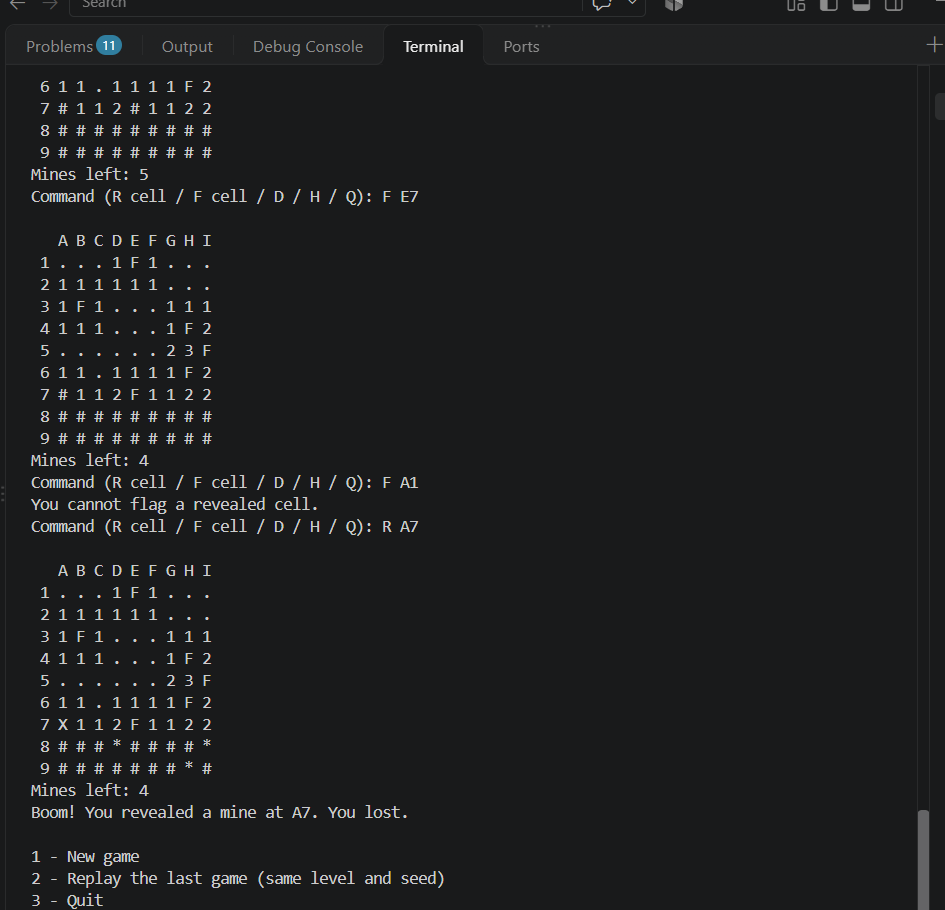
\includegraphics[width=0.52\linewidth]{photos/our_game_loss.png}
\caption{Our game in the VS Code terminal: \code{F A1} on a revealed cell is refused, then \code{R A7} hits a mine.}
\label{fig:vscode}
\end{figure}

{\footnotesize
\renewcommand{\arraystretch}{1.1}
\begin{longtable}{>{\bfseries}l p{3.2cm} p{3.6cm} p{3.4cm} p{3.6cm}}
\toprule
\textbf{ID} & \textbf{Test} & \textbf{Input} & \textbf{Expected} & \textbf{Obtained}\\
\midrule
\endhead
T1 & First move is always safe & R <any cell>, 1200 games + 20 real runs & never a mine & 0 mines hit in 1220 games -- pass\\
T2 & Flood fill opens the empty area & seed 7, R E5 & same board as the example of the assignment & identical to the example, 40 cells opened -- pass\\
T3 & Flag on a revealed cell & R E5 then F E5 & error message, turn kept & ``You cannot flag a revealed cell.'' -- pass\\
T4 & Cell outside the board & R Z99, R J1, R A10, R A0 & error message, ask again & ``Cell outside the board.'' 4 times -- pass\\
T5 & Badly written cell & R E, R 5E, R E-5, R E5.0, R E$^2$ & error message, no crash & ``Invalid cell...'' five times -- pass\\
T6 & Unknown, empty or incomplete command & empty line, hello, X E5, R, R E5 E6, D 3 & clear message for each, no crash & 6 different messages, exit code 0 -- pass\\
T7 & Reveal an already revealed cell & R E5, R E5, R F3 & error message, turn kept & ``This cell is already revealed.'' -- pass\\
T8 & Reveal a flagged cell & F A1 then R A1 & refused, flag must be removed & ``This cell has a flag. Remove the flag first (F).'' -- pass\\
T9 & Put and remove a flag & F A1, F A1 & F appears then disappears; 10 $\rightarrow$ 9 $\rightarrow$ 10 & Mines left 10 $\rightarrow$ 9 $\rightarrow$ 10 -- pass\\
T10 & Lower case and extra spaces & ``   r   e5  '' & same as R E5 & accepted, same board as T2 -- pass\\
T11 & Win & seed 7, reveal the 71 safe cells & win message + full board & ``Congratulations, you won!'', all mines shown -- pass\\
T12 & Loss & seed 7, R E5 then R G1 & X on G1, * on the other mines & ``Boom! ... at G1'', X on G1, 9 x * -- pass\\
T13 & Wrong flag shown at the end & F A1 (no mine), F H1 (mine), then lose & ! on A1, F kept on H1 & A1 = !, H1 = F -- pass\\
T14 & Flood fill does not open a flag & F I5 then R E5 & I5 stays F, area opened & I5 = F, neighbours opened -- pass\\
T15 & Replay gives the same board & menu 2 after a game, same first move & identical boards & identical boards -- pass\\
T16 & Debug mode & D before and after the first move & message, then 10 mines shown, game continues & 10 x * shown, next command accepted -- pass\\
T17 & Hard level 16 x 16 & R P16, R Q1 & P16 accepted, Q1 outside, rows aligned & 16 aligned rows, Q1 refused -- pass\\
T18 & Invalid menu, level and seed & 9, 2 (no game yet), 0, 5, abc, -5 & asked again each time & asked again 6 times -- pass\\
T19 & Help, quit game, quit program & h, q, 3 & help shown, back to menu, program ends & help, ``Game stopped.'', ``Goodbye!'' -- pass\\
T20 & No seed given & Enter at the seed question & random seed shown, replay identical & seed shown, replay identical -- pass\\
F1 & Fuzz: random text to parse\_command & 50 000 random strings & no exception & 0 exceptions -- pass\\
F2 & Fuzz: 1500 random games & random reveals and flags & no mine or flag ever revealed & 0 rule violations -- pass\\
E1 & Hint command (extra) & HINT before and after R E5; 300 Hard games solved by hints only & message, then a safe cell & ``Hint: D1 is safe.''; 300/300 games won with hints -- pass\\
E2 & Timer and best times saved in a file (extra) & win, quit, restart, menu 4 & time shown, record kept after restart & time shown, scores.txt read back -- pass\\
E3 & Badly written score file (extra) & file with wrong lines & wrong lines ignored & only the valid line shown -- pass\\
E4 & Custom board size (extra) & 4, 21, abc, 20, 20, 101, 0, 100 & asked again; 20 x 20 with 100 mines & 3 + 2 refusals, 20 x 20 board, 100 mines -- pass\\
\bottomrule
\end{longtable}}

% ------------------------------------------------------------------ 7
\section{Difficulties and solutions}

\begin{center}
\small
\begin{tabularx}{\linewidth}{l X X}
\toprule
& \textbf{Problem} & \textbf{Solution}\\
\midrule
1 & \code{str.isdigit()} accepts characters such as the superscript two (\code{\textsuperscript{2}}),
  but \code{int()} cannot convert them: \code{R E\textsuperscript{2}} would crash the program. &
  Our own function \code{is\_number()} accepts only the characters \code{0}--\code{9}.\\
2 & Mines must be random but the same seed must give the same board. Taking cells from a
  \emph{set} would not guarantee the same order. &
  \code{place\_mines} builds the candidates in a \emph{list}, row by row, and \code{start\_mines}
  calls \code{random.seed(seed)} just before \code{random.sample}.\\
3 & First version: \code{Q} closed the whole program, but the assignment says \emph{quit the
  current game}. & \code{Q} now returns to the menu (new game, replay, quit).\\
4 & Without a seed a game could not be replayed. & The program chooses a random seed and shows it;
  menu option 2 replays it.\\
5 & The first board layout and prompt did not match the example screen of the assignment
  (extra spaces, different prompt). & Header, spacing and prompt changed to match it; row numbers are
  right-aligned on 2 characters (\code{rjust(2)}) so rows 1--9 line up with 10--16 (test T17).\\
6 & The first move must be safe, but the mines must exist to compute the numbers. &
  The mines are placed inside \code{reveal}, at the first call, excluding the chosen cell
  (test T1: 1\,220 games, no mine hit).\\
7 & A cell can be pushed several times on the stack (Section 4). &
  It is skipped when it is popped if it is already revealed.\\
8 & Two non-ASCII characters (\code{\textsuperscript{2}} and a long dash) in comments could be shown
  wrongly with some Windows encodings. & All files now contain only ASCII characters.\\
9 & \textbf{Known limitation.} If the input stream is closed (Ctrl+Z then Enter on Windows,
  Ctrl+D on Linux), \code{input()} raises an error. &
  Catching it needs \code{try}/\code{except}, which is not in the list of allowed notions; normal
  typing can never cause it.\\
\bottomrule
\end{tabularx}
\end{center}

% ------------------------------------------------------------------ 8
\needspace{12\baselineskip}
\section{Contributions}

Each member is responsible for at least two functions and can explain and modify them. Everyone
took part in studying the game, in the tests and in this report.

\begin{center}
\small
\begin{tabularx}{\linewidth}{l X X}
\toprule
\textbf{Member} & \textbf{Functions} & \textbf{Report}\\
\midrule
Zeynalzada Ayxan & \code{play\_game}, \code{check\_win}, \code{check\_loss}, \code{new\_state},
  \code{cell\_name}, \code{main}, \code{ask\_menu}; extra: timer and \code{scores.py} &
  coordination, overview, main-loop flowchart, test plan\\
Nuruzada Nihat & \code{create\_board}, \code{place\_mines}, \code{start\_mines},
  \code{choose\_level} & design, data structures, seed\\
Qurbanli Elton & \code{neighbours}, \code{count\_adjacent}, \code{compute\_numbers};
  extra: custom board size & complexity analysis\\
Maharramli Anvar & \code{reveal}, \code{toggle\_flag}; extra: \code{find\_hint} &
  reveal flowchart, $5\times5$ trace\\
Hamzayev Altair & \code{display\_board}, \code{cell\_symbol}, \code{parse\_command},
  \code{parse\_cell}, \code{is\_number}, \code{show\_help} & user interface, difficulties\\
\bottomrule
\end{tabularx}
\end{center}

% ------------------------------------------------------------------ 9
\section{Optional extras}\label{sec:extras}

The extras were added only after all mandatory tests passed, and they do not change the
mandatory behaviour (tests T1--T20 still pass).
\begin{itemize}
\item \textbf{\code{HINT} command.} \code{find\_hint} returns a safe hidden cell, preferably next to the
  revealed area. Test E1 solved 300 Hard games using only hints, without hitting a mine.
\item \textbf{Timer and scoreboard.} \code{play\_game} measures the time with \code{time.time()} and
  returns it when the game is won. The best time of each board is kept in a \emph{dictionary}
  (key \code{"9x9, 10 mines"}) shown with menu option 4.
\item \textbf{Scoreboard saved in a file.} The dictionary is written to \code{scores.txt} (one
  \code{key;seconds} per line) and read back at start. The file is opened with mode \code{"a+"},
  which creates it if it does not exist, so no error is possible; wrong lines are ignored (test E3).
\item \textbf{Custom board size.} Level 4 asks rows and columns from 5 to 20 and at most 25\,\% of
  mines, and asks again until the values are valid (test E4).
\end{itemize}
We did not add the ``safer first move'' extra, because it would change the boards: the demonstration
board of the assignment (seed 7) would no longer be reproduced. Colours and a graphical interface
were not added either.

\end{document}
